\documentclass[12pt, letterpaper]{article}
\usepackage[spanish]{babel}
\usepackage[utf8]{inputenc}
\usepackage{graphicx}
\usepackage{amssymb}
\graphicspath{{./imagenes/}}

%Paquetes para símbolos y entornos matematicos. En este documento se usa para poder usar el tag \begin{align} y \begin{align*} que permiten alinear expresiones matemáticas
\usepackage{amsmath}
\usepackage{amssymb}
%paquete que permite el uso de del argumento H al momento de insertar imágenes
\usepackage{float}
\usepackage{xcolor}

%comando para especificar el título del documento 
\title{Matemáticas para las Ciencias Aplicadas I}

%comando para especificar el autor del documento
\author{Pérez Romero Natalia Abigail}

%comando para especificar la fecha del documento
\date{\today}
%--------------Fin preámbulo--------------

%------------Inicio documento-------------
\begin{document}
%comando que genera el titulo con los datos especificados en el preámbulo
\maketitle
\textbf{Tarea V. Ejercicios del libro Cálculo. Una variable de Thomas J.R, George B.}

\textbf{Ejercicios 11, 15 y 18}

\textbf{Funciones crecientes y decrecientes}
Trace las gráficas de las funciones. ¿Qué simetrías tiene las gráficas? Especifique los intervalos en donde la función es creciente y los intervalos donde es decreciente.

(11) $y = \sqrt{|x|}$

Una gráfica es simétrica respecto al eje $y$ si es par. 
Se dice que una función es par si $f(-x)=f(x)$

Consideramos: 
$f(-x)$ , $x = 1$
\begin{align*}
	f(-1) &=  \sqrt{|-1|}\\
	f(-1) &= \sqrt{1}\\
	f(-1) &= 1
\end{align*}

$f(x)$ , $x = 1$
\begin{align*}
	f(1) &=  \sqrt{|1|}\\
	f(1) &= \sqrt{1}\\
	f(1) &= 1
\end{align*}

Como $f(-1)= f(1)$ la función $f(x) = \sqrt{|x|}$ es par

\begin{figure}[h]
\centering
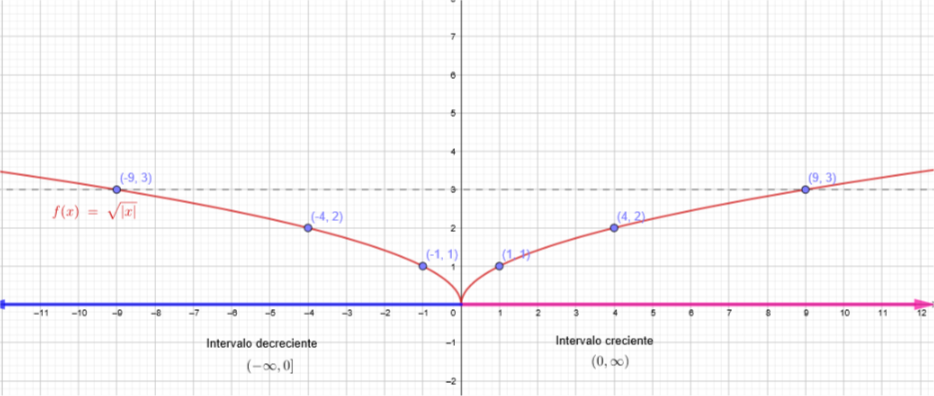
\includegraphics[width=30em]{creceuno}
\end{figure}

\newpage

(15) $y= -x^{\frac{3}{2}}$

Una gráfica es simétrica respecto al eje $y$ si es par. 
Se dice que una función es par si $f(-x)=f(x)$

Consideramos: $f(x)$ , $x = 1$
\begin{align*}
	f(1) &=  (-1)^{\frac{3}{2}}\\
	f(1) &= -1
\end{align*}

Sin embargo $f(x)$ no está definida en los reales para $x = -1$ por lo que la función no es simétrica con respecto al eje $y$  

\begin{figure}[h]
\centering
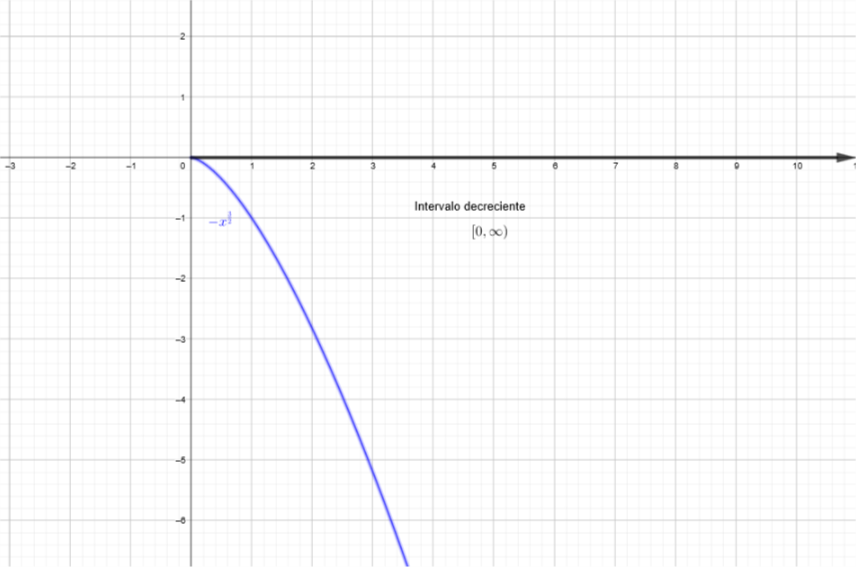
\includegraphics[width=30em]{crecedos}
\end{figure} 
\newpage

(18) $y= -x^{\frac{2}{3}}$

\begin{figure}[h]
\centering
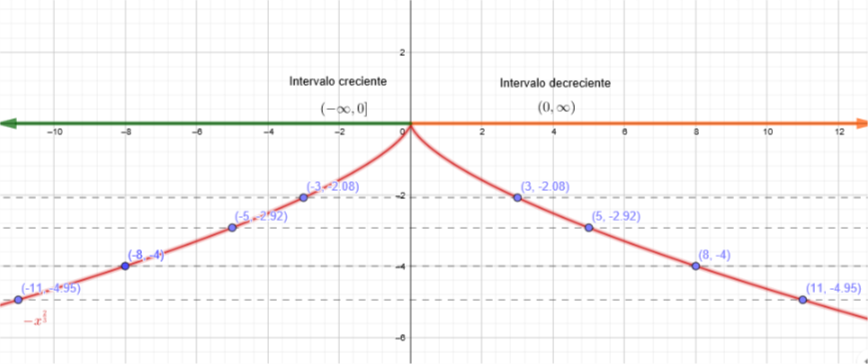
\includegraphics[width=30em]{crecetres}
\end{figure}

Una gráfica es simétrica respecto al eje $y$ si es par. 
Se dice que una función es par si $f(-x)=f(x)$

Consideramos: $f(x)$ , $x = 3$
\begin{align*}
	f(3) &=  -(3)^{\frac{3}{2}}\\
	f(3) & \approx -2.080
\end{align*}

$f(-x)$ , $x = -3$
\begin{align*}
	f(-3) &=  -(-3)^{\frac{3}{2}}\\
	f(-3) & \approx -2.080
\end{align*}

Como $f(-3)= f(3)$ la función $f(x) = -x^{\frac{2}{3}}$ es par

\newpage

\textbf{Proporcionalidad. Actividad 32.}
\hfill \break
Evalúe si el conjunto de datos dados satisfacen razonablemente la suposición de proporcionalidad señalada. Trace un diagrama de dispersión apropiado para su investigación y, si la hipótesis de proporcionalidad parece razonable, estime la constante de proporcionalidad.


a. $y$ es proporcional respecto a $3^x$

\begin{tabular}{c|c|c|c|c|c|c|c|c}
x & 5 & 15 & 45 &135 & 405 & 1215& 3645 & 10,935\\
\hline
y & 0 & 1 & 2 & 3 & 4 & 5 & 6 & 7 
\end{tabular}

Si solo se considerará $3^x$ no parece existir proporcionalidad
\begin{align*}
	3^0 = 1 \neq 5\\
	3^1 = 3 \neq 15\\
	3^3 =9 \neq 135\\
	3^6 = 729 \neq 3645\\
	3^7 = 2187 \neq 10935
\end{align*}

Sin embargo, al observar los casos anteriores se puede hipotizar que si es proporcional y la constante es 5:
\begin{align*}
	(3^0)*5  = 5\\
	(3^1)*5 = 15\\
	(3^3)*5 = 27*5 = 135\\
	(3^6)*5 = 729*5 = 3645\\
	(3^7)*5 = 2187*5 = 10935
\end{align*}

Ahora si coinciden los resultados $\therefore$ la constante de proporcionalidad debe ser 5

\begin{figure}[h]
\centering
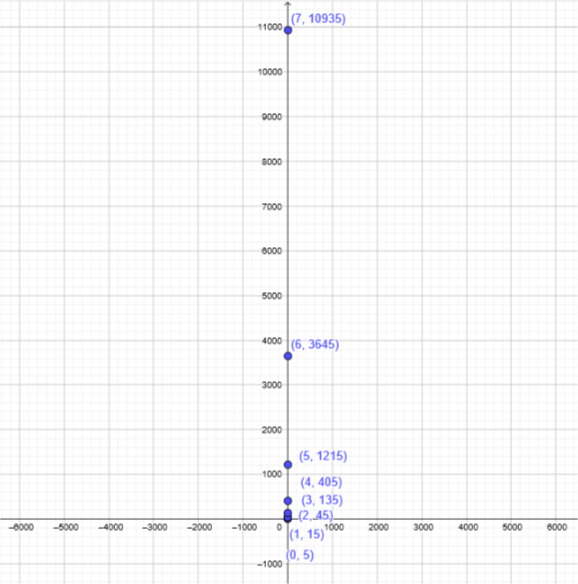
\includegraphics[width=30em]{crececuatrosuno}
\end{figure}
 
\newpage
b. $y$ es proporcional respecto a $x$

\begin{tabular}{c|c|c|c|c|c|c|c|c}
x & 2 & 4.8 & 5.3 & 6.5 & 8.0 & 10.5 & 14.4 & 15.0\\
\hline
y & 2.0 & 5.0 & 6.0 & 9.0 & 14.0 & 35.0 & 120.0 & 150.0 
\end{tabular}

No existe proporcionalidad, para comprobar esto elaboré una tabla en la que registre el cambio observado y comparé con el cambio esperado de $x$ para $y$
\newpage
\begin{table}[htb]
\centering
\begin{tabular}{|p{1.2cm}|c|c|c|c|c|c|c|c|c|c|c|c|c|}
\hline
x & 2.0 & 3.0 & 4.0 & 5.0 & 6.0 & 7.0 & 8.0 & 9.0 & 10.0 & 11.0 & 12.0 & 13.0 & 14.0\\
\hline
y & 2    & x   &  x   & 4.8 & 5.3 &   x &    x & 6.5 &   x   &  x    &  x    &   x    & 8.0\\
\hline
cambio observado & 0    & x   &  x   & -0.2 & -0.7 &   x &    x & -2.5 &   x   &  x    &  x    &   x    & -6\\
\hline
\end{tabular}
\end{table}
A partir de observo que de -0.7 a -0.2 hay un cambio de -0.5 así que mi  tabla queda así:

\begin{table}[htb]
\centering
\begin{tabular}{|p{1.2cm}|c|c|c|c|c|c|c|c|c|c|c|c|c|}
\hline
x & 2.0 & 3.0 & 4.0 & 5.0 & 6.0 & 7.0 & 8.0 & 9.0 & 10.0 & 11.0 & 12.0 & 13.0 & 14.0\\
\hline
y & 2    & x   &  x   & 4.8 & 5.3 &   x &    x & 6.5 &   x   &  x    &  x    &   x    & 8.0\\
\hline
cambio observado & 0    & x   &  x   & -0.2 & -0.7 &   x &    x & -2.5 &   x   &  x    &  x    &   x    & -6\\
\hline
cambio esperado & \textcolor{red}{1.3} & 0.8  &  0.3   & -0.2 & -0.7 &  -1.2 &    -1.7 & \textcolor{red}{-2.2} &   -2.7   &  -3.2    &  -3.7    &   -4.2    & \textcolor{red}{-4.7}\\
\hline
\end{tabular}
\end{table}

Como se observa en la tabla mis predicciones fueron incorrectas, por lo que este cambio no resulta útil.

Tambien observo que no hay ninguna relacion ente la $x$ y su cambio en $y$ por ejemplo:

\begin{align*}
	6 / 5.3  \approx 1.132\\
	5 / 4.8  \approx 1.0416\\
	9 / 6 = 1.5\\
	14 / 8  = 1.75\\
	120 / 14.4  \approx 8.33\\
	150 / 15  = 10
\end{align*}

$\therefore y$ no es proporcional respecto a $x$

\begin{figure}[t]
\centering
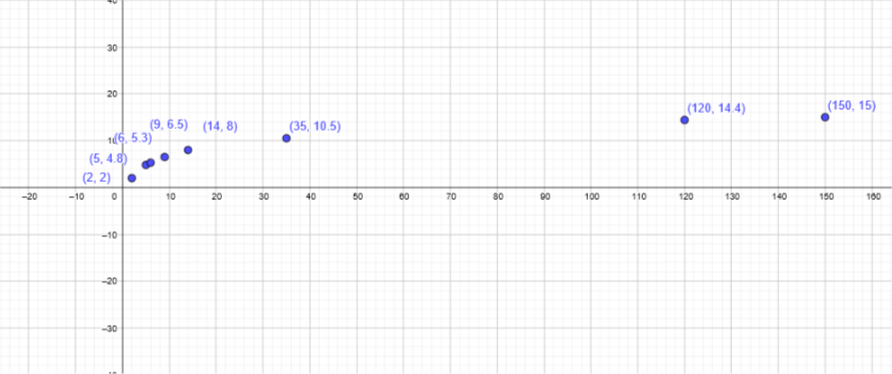
\includegraphics[width=40em]{crececinto}
\end{figure}



\end{document}
%----------Fin del documento--------------